\documentclass{exam}
\usepackage[utf8]{inputenc}
\usepackage{systeme,mathtools}
\usepackage{amssymb,amsmath,amsthm}
\usepackage{bbm}
\usepackage{algorithm}
\usepackage{algorithmic}
\usepackage{graphicx}
\usepackage[francais]{babel}
\usepackage{fontspec}
\usepackage{systeme}
\begin{document}
\newcommand{\espace}{\vspace{0.5cm}}
\newcommand{\increment}{\hspace{0.5cm}}

1) Soit $\mathbb{Q}$ une probabilité telle que sous cette probabilité on a $E_{\mathbb{Q}}[T_1^{(N)}] = 1 + r_N$. Ainsi : 
\newline
\espace
$E_{\mathbb{Q}}[T_1^{(N)}] = 1 + r_N=\underset{x \in \{1+h_N,1+b_N\}}{\sum} x \mathbb{Q}(T_1^{(N)}=x)=(1+h_N)q_N + (1+b_N)(1-q_N)$
\newline
\espace
Ainsi, on obtient :
$$\boxed{q_N = \frac{r_N - b_N}{h_N - b_N}}$$

On remarque que l'on a bien $q_N \in [0,1]$.
\newline
\espace
2) Déterminons le prix de l'option $p_{(N)}$ de l'option qui paye $f(S_{t_N}^{(N)})$.

Pour $i \in \{1,..,N\}$, posons $X_i=\mathbbm{1}_{T_i^{(N)}=1+h_N}$. Il est facile de montrer que $X_i$ suit une loi de Bernoulli de paramètre $q_N$. Posons $Y_N=\underset{1 \leq i \leq N }{\sum}X_i$. Les variables aléatoires $(T_i^{(N)})_{1 \leq i \leq N}$ étant indépendantes et identiquement distribuées, il en est de même pour les variables aléatoires $(X_i^{(N)})_{1 \leq i \leq N}$. On reconnait ainsi que $Y_N$ est une loi binomiale de paramètres $N$ et $q_N$. On remarque enfin que $P_{\mathbb{Q}}(S_{t_N}^{(N)}=s(1+h_N)^k(1+b_N)^{N-k})=P_{\mathbb{Q}}(Y_i=k)=C_N^k q_N^k (1-q_N)^{N-k}$. Ainsi, par le théorème de transfert :
\newline
\espace
$p_{(N)}=\frac{1}{(1+r_N)^N}\mathbb{E}_{\mathbb{Q}}[f(S_{t_N}^{(N)})]=\frac{1}{(1+r_N)^N}\overset{N}{\underset{k=0}{\sum}}f(s(1+h_N)^k(1+b_N)^{N-k})P_{\mathbb{Q}}(S_{t_N}^{(N)}=s(1+h_N)^k(1+b_N)^{N-k})$
\newline
\espace
Ce qui donne :
$$\boxed{p_{(N)}=\frac{1}{(1+r_N)^N}=\overset{N}{\underset{k=0}{\sum}}f(s(1+h_N)^k(1+b_N)^{N-k})C_N^k q_N^k (1-q_N)^{N-k}}$$
\newline
\espace
3) \begin{algorithm}
\caption{price1($N,r_N,h_N,b_N,s,f$)}
\begin{algorithmic}
\ENSURE $res \times sum = p_{(N)}$
\STATE $q_N \leftarrow \frac{r_N-b_N}{h_N-b_N}$
\STATE $res \leftarrow \frac{1}{(1+r_N)^N}$
\STATE $sum \leftarrow 0$
\FOR{k in 0:N}
\STATE $sum \leftarrow sum + f(s(1+h_N)^k(1+b_N)^{(N-k)})C_N^kq_N^k(1-q_N)^{(N-k)}$
\ENDFOR
\end{algorithmic}
\end{algorithm}
\newline
\espace
4) Voir code python.
\newline
\espace
5)On sait que $\mathbb{E}_\mathbb{Q}[v_{k+1}(S_{t_{k+1}}^{(N)})|S_{t_k}^{(N)}]=v_{k+1}((1+h_N)S_{t_k}^{(N)})q_N + v_{k+1}((1+b_N)S_{t_k}^{(N)})(1-q_N)$. Ainsi :
\begin{algorithm}
\caption{price2($N,r_N,h_N,b_N,s,f,k$)}
\begin{algorithmic}
\ENSURE res = $p_{(N)}$
\IF{$k = N$}
\STATE $res \leftarrow f(s)$
\ELSE
\STATE $q_N \leftarrow \frac{r_N-b_N}{h_N-b_N}$
\STATE $esp \leftarrow price2(N,r_N,h_N,b_N,s(1+h_N),f,k+1)q_N + price2(N,r_N,h_N,b_N,s(1+b_N),f,k+1)(1-q_N)$
\STATE $res \leftarrow \frac{esp}{1+r_N}$
\ENDIF
\end{algorithmic}
\end{algorithm}
\newline
\espace
6)
\newline
\espace
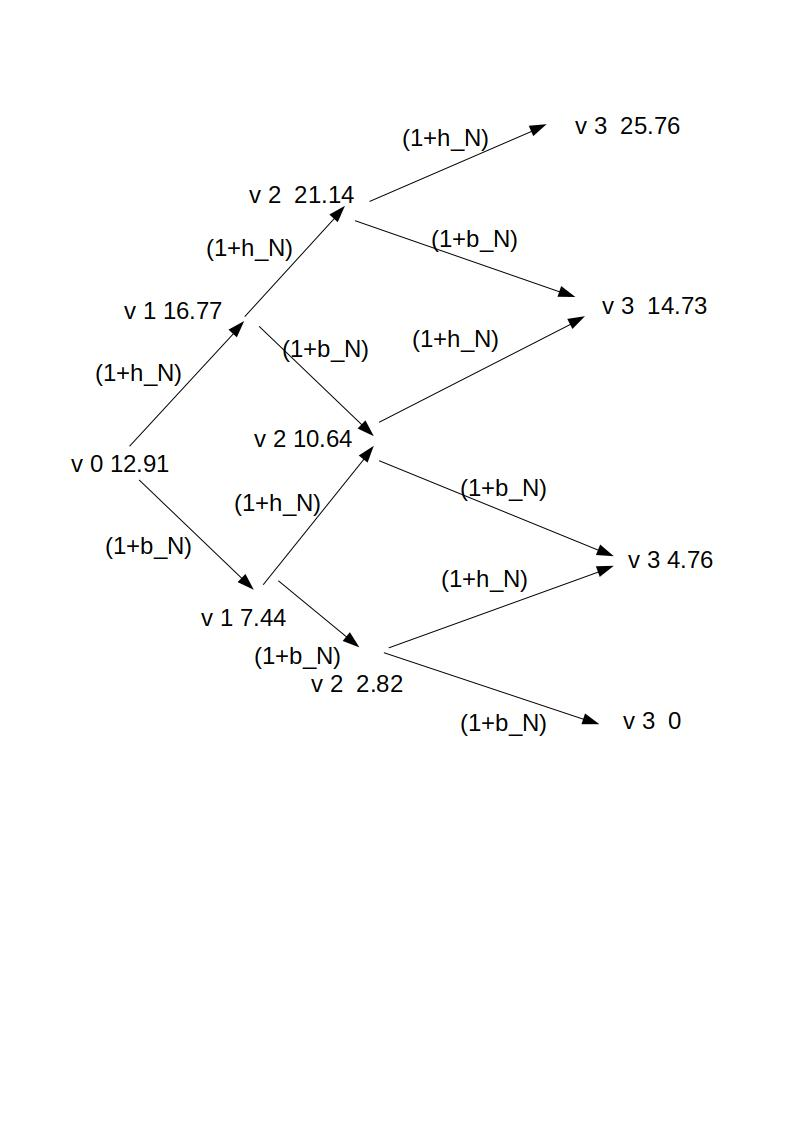
\includegraphics{question6tree.jpg}
\newline
\espace
7)
\newline
\espace
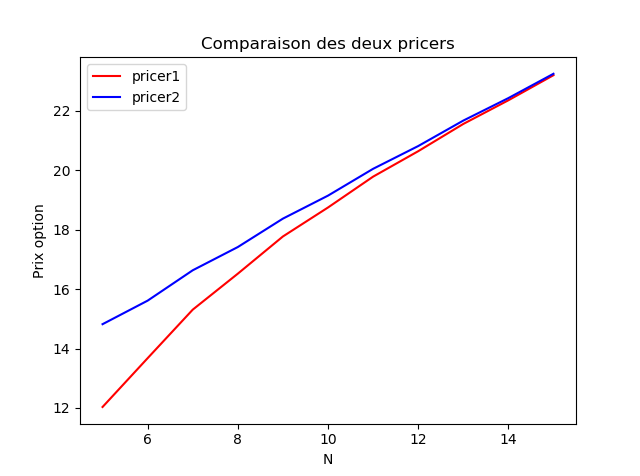
\includegraphics{question7.png}
\newline
\espace
8) Le système à la date $t_N$ vaut :
\newline
\vspace{0.5cm}
$\alpha_{N-1}(S_{t_{N-1}}^{(N)})(1 + h_N)S_{t_{N-1}}^{(N)} + \beta_{N-1}(S_{t_{N-1}}^{(N)})S_{t_N}^{0} = f((1+h_N)S_{t_{N-1}}^{(N)})$ \hspace{1cm} [1]
\newline
\vspace{0.5cm}
$\alpha_{N-1}(S_{t_{N-1}}^{(N)})(1+b_N)S_{t_{N-1}}^{(N)} + \beta_{N-1}(S_{t_{N-1}}^{(N)})S_{t_N}^{0} = f((1+b_N)S_{t_{N-1}}^{(N)})$ \hspace{1cm} [2]
\newline
\vspace{0.5cm}
$[1]-[2]$ donne :
\newline
\vspace{0.5cm}
$\alpha_{N-1}(S_{t_{N-1}}^{(N)})=\frac{f((1+h_N)S_{t_{N-1}}^{(N)})-f((1+b_N)S_{t_{N-1}}^{(N)})}{(h_N-b_N)S_{t_{N-1}}^{(N)}}$
\newline
\vspace{0.5cm}
$(1+h_N)[1]-(1+b_N)[2]$ donne:
\newline
\vspace{0.5cm}
$\beta_{N-1}(S_{t_{N-1}}^{(N)})=\frac{1}{S_{t_N}^0(h_N-b_N)}(f((1+b_N)S_{t_{N-1}}^{(N)})(1+h_N)-f((1+h_N)S_{t_{N-1}}^{(N)})(1+b_N))$
\newline
\vspace{0.5cm}
9) Le système pour les autres dates $t_k$ vaut :
\newline
\vspace{0.5cm}
$\alpha_{k-1}(S_{t_{k-1}}^{(N)})(1 + h_N)S_{t_{k-1}} + \beta_{k-1}(S_{t_{k-1}}^{(N)})S_{t_k}^{0} = v_k((1+h_N)S_{t_{k-1}}^{(N)})$ \hspace{1cm} [1]
\newline
\vspace{0.5cm}
$\alpha_{k-1}(S_{t_{k-1}}^{(N)})(1+b_N)S_{t_{k-1}} + \beta_{k-1}(S_{t_{k-1}}^{(N)})S_{t_k}^{0} = v_k((1+b_N)S_{t_{k-1}}^{(N)})$ \hspace{1cm} [2]
\newline
\vspace{0.5cm}
Ce qui donne, par un raisonnement analogue : 
\newline
\vspace{0.5cm}
$\alpha_{k-1}(S_{t_{k-1}}^{(N)})=\frac{v_k((1+h_N)S_{t_{k-1}}^{(N)})-v_k((1+b_N)S_{t_{k-1}}^{(N)})}{(h_N-b_N)S_{t_{k-1}}^{(N)}}$
\newline
\vspace{0.5cm}
$\beta_{k-1}(S_{t_{k-1}}^{(N)})=\frac{1}{S_{t_k}^0(h_N-b_N)}(v_k((1+b_N)S_{t_{k-1}}^{(N)}(1+h_N)-v_k((1+h_N)S_{t_{k-1}}^{(N)}(1+b_N))$
\newline
\vspace{0.5cm}
10) Voir code pyton.
\newline
\vspace{0.5cm}
11) En appliquant la formule d'Ito à $ln (S_t)$, on obtient :
\newline
\espace
$dln(S_t)=\frac{1}{S_t}dS_t + \frac{1}{2}(\sigma S_t)^{2}(-\frac{1}{S_t^{2}})dt$  
\newline
\espace
\Longleftrightarrow \hspace{0.5cm} $dln(S_t)=(r dt + \sigma dB_t)-\frac{\sigma^{2}}{2} dt$ \hspace{0.5cm} car \hspace{0.5cm} $dS_t=S_t(rdt + \sigma dB_t)$
\newline
\espace
\Longleftrightarrow \hspace{0.5cm} $dln(S_t)=(r-\frac{\sigma^2}{2})dt + \sigma dB_t$
\newline
\espace
\Longleftrightarrow \hspace{0.5cm} $lnS_t - lns$ = $(r-\frac{\sigma^2}{2})t + \sigma B_t$ \hspace{0.5cm} car $B_0=0$
\newline
\espace
Soit au final:
\newline
\espace
$$\boxed{S_t=s \exp{(\sigma B_t + (r-\frac{\sigma^2}{2})t)}}$$
\newline
\espace
12)
\newline
\espace
13) 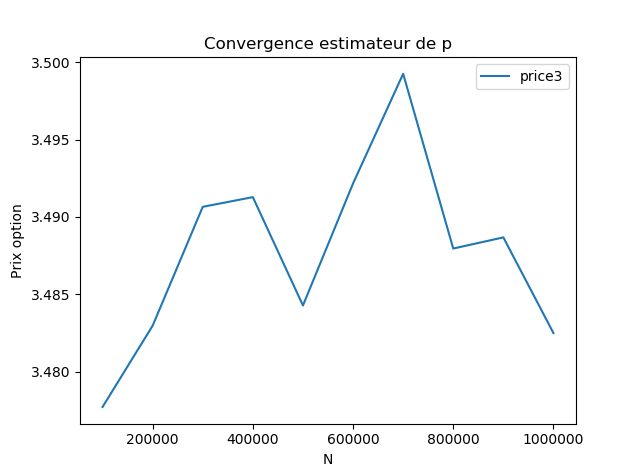
\includegraphics{question13.png}
\newline
\espace
14) Posons pour $1 \leq i \leq n, X_i = e^{-rT}f(s \exp ((r-\frac{\sigma^2}{2})T + \sigma \sqrt{T} \epsilon_i)$. Pour montrer que la suite $(\hat{p}_{(n)})_{n \in \mathbb{N}}$ converge presque sûrement vers $p$, il suffit de montrer que E[$X_0$]=$p$. En effet, les $(\epsilon_i)_{1 \leq i \leq n}$ étant indépendantes et identiquement distribuées, il en de même pour les $(X_i)_{1 \leq i \leq n}$. E[$X_0$]=$p < +\infty$ permet de conclure, d'après la loi forte des grands nombres, que la suite $(\hat{p}_{(n)})_{n \in \mathbb{N}}$ converge presque sûrement vers $p$. 

Or d'après les propriétés 1 et 2 du mouvement brownien énoncées dans le sujet, on sait que $B_t \sim N(0,t)$, donc que $\frac{B_t}{\sqrt{t}} \sim N(0,1)$. On en déduit qu'il existe $\varepsilon^{'} \sim N(0,1)$ tel que pour tout T, on a $B_T = \sqrt{T}\varepsilon^{'}$. $\varepsilon^{'}$ et les $(\epsilon_i)_{1 \leq i \leq n}$ étant de même loi, on en déduit que  E[$X_0$]=$p$.
\newline
\espace
15)
\newline
\espace
16) Voir code python.
\newline
\espace
17) 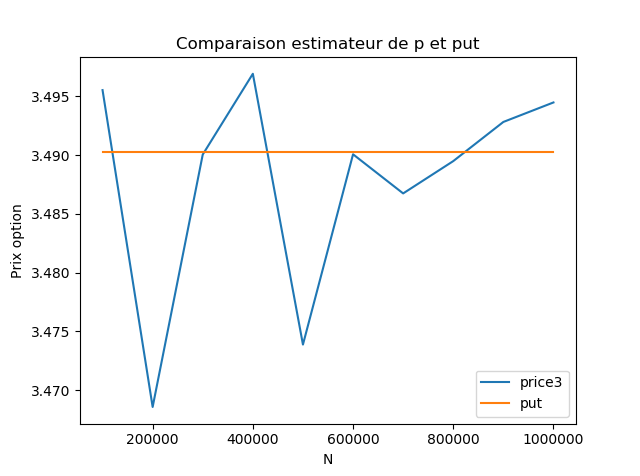
\includegraphics{question17.png}
\newline
\espace
18) 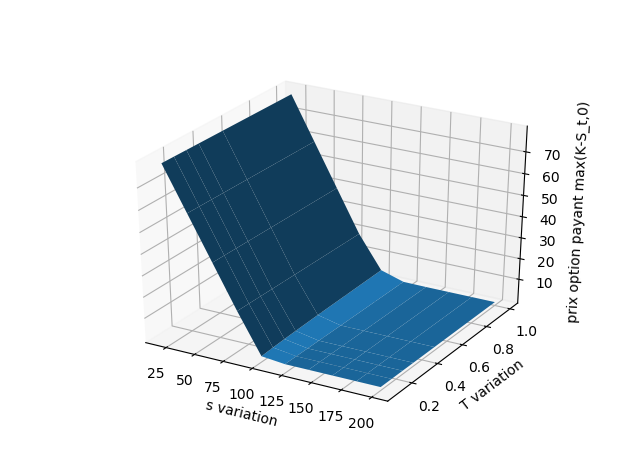
\includegraphics{question18.png}
\newline
\espace
19)
\newline
\espace
20)

\end{document}
